\documentclass{article}
\usepackage{graphicx} % Required for inserting images
\usepackage{graphicx} % Required for inserting images
%\usepackage[left=0.5in, right=0.5in, top=0.5in, bottom=0.5in]{geometry}
\usepackage[left=1cm, right=1cm, top=0.5cm, bottom=1.5cm]{geometry}
\usepackage{amsmath}
\usepackage{amssymb}
\usepackage{amsfonts}
\usepackage{amsthm}
\usepackage{ulem}
\usepackage{bm}
\usepackage{tikz}

% \title{Fractions, Decimals and Percentage}
\date{}

\begin{document}
\fontsize{13}{15} \selectfont %This is 14pt text with 16pt line spacing.

\begin{center}
    
 \text{Place Value 1.} \qquad \\ 
\end{center} \\ 
Name: \hspace{8cm}  Date: \hspace{4cm} Class: \hspace{2cm}  

\par
\vspace*{10pt} 
\textit{(You must show your working.)  }
\vspace{10pt}

\hline
\vspace{10pt}

\par
\text{(1) What is 248523 rounded to the nearest ten thousand? } \\
\vspace*{20pt}
\par

\begin{flushright}
    \text{ (2)}
\end{flushright}
 \vspace{10pt}

\hline
\vspace{10pt}

\par
\text{(2) Write these numbers in order of size. Start with the smallest. } \\

2.36 \hspace{3cm} 3.26 \hspace{3cm} 2.6 \hspace{3cm} 2.63 \hspace{3cm} 2.3 
\vspace{60pt}

 ..... \hspace{3cm} ..... \hspace{3cm}  ..... \hspace{3cm} ..... \hspace{3cm} .....  

\par
\text{smallest} 
\vspace{10pt}
\begin{flushright}
    \text{ (2)}
\end{flushright}
 \vspace{10pt}

\hline
\vspace{10pt}
\par
\text{(3) Write these numbers in order of size. Start with the smallest. } \\

0.45 \hspace{3cm} 0.72 \hspace{3cm} 26\% \hspace{3cm}  \( \displaystyle \frac{7}{10} \) 
\vspace{60pt}

 ..... \hspace{3cm} ..... \hspace{3cm}  ..... \hspace{3cm} .....    } \\

 smallest
 
 \begin{flushright}
    \text{ (2)}
\end{flushright}
 
 \vspace{10pt}
 \hline
 \vspace{10pt}

  %\begin{figure}[h]
      %
\includegraphics[width=1cm\textwidth]{cross.png}
%\end{figure}

 %\begin{figure}[h]
      %
\includegraphics[width=1cm]{cross.png} \hspace{3cm} 
%\end{figure}

 %\begin{figure}[h]
      %
\includegraphics[width=1cm]{cross.png}\hspace{3cm} 
%\end{figure}

 %\begin{figure}[h]
      %
\includegraphics[width=1cm]{cross.png}\hspace{3cm} 
%\end{figure}

%
\includegraphics[width=1cm]{cross.png} \hfill
%
\includegraphics[width=1cm]{cross.png} \hfill
%
\includegraphics[width=1cm]{cross.png} \hfill
%
\includegraphics[width=1cm]{cross.png}

%\textbf{Question 1:} Choose your preferred answer:

%\begin{center}
%\begin{tabular}{cccc}
  %Ones & Tens & Hundreds & Tenths \\
 % 
\includegraphics[width=1cm]{cross.png} & 
  %
\includegraphics[width=1cm]{cross.png} & 
  %
\includegraphics[width=1cm]{cross.png} & 
 % 
\includegraphics[width=1cm]{cross.png} \\
%\end{tabular}
%\end{center}

%\text{(4) What does 7 represent in this number?   } \\
 %\[ 62.37\]
 %\text{ Ones \hspace{3cm} Tens \hspace{3cm} Hundreds \hspace{3cm}} Tenths } \\ 

%\begin{center}
%\begin{tabular}{cccc}
  %Ones & Tens & Hundreds & Tenths \\
  %
\includegraphics[width=1cm]{cross.png} & 
  %
\includegraphics[width=1cm]{cross.png} & 
  %
\includegraphics[width=1cm]{cross.png} & 
 % 
\includegraphics[width=1cm]{cross.png} \\
%\end{tabular}
%\end{center}

%\text{(4) What does 7 represent in this number?   } \\
 %\[ 62.37\]
 %\text{ Ones \hspace{3cm} Tens \hspace{3cm} Hundreds \hspace{3cm}} Tenths } \\ 


\text{(4) What does 7 represent in this number?   } \\
 \[ 62.37\]
 
\begin{center}
\begin{tabular}{c@{\hspace{3cm}}c@{\hspace{3cm}}c@{\hspace{3cm}}c}
  Ones & Tens & Hundreds & Tenths \\
  
\includegraphics[width=1cm]{cross.png} & 
  
\includegraphics[width=1cm]{cross.png} & 
  
\includegraphics[width=1cm]{cross.png} & 
  
\includegraphics[width=1cm]{cross.png} \\
\end{tabular}
\end{center}

\begin{flushright}
    \text{ (2)}
\end{flushright}
 \vspace{10pt}
 \newpage

\text{(5) What is 7358 rounded to the nearest hundred? }
\begin{center}
\begin{tabular}{c@{\hspace{3cm}}c@{\hspace{3cm}}c@{\hspace{3cm}}c}
  7000 & 7300 & 7400 & 8000 \\
  
\includegraphics[width=1cm]{cross.png} & 
  
\includegraphics[width=1cm]{cross.png} & 
  
\includegraphics[width=1cm]{cross.png} & 
  
\includegraphics[width=1cm]{cross.png} \\
\end{tabular}
\end{center}

\begin{flushright}
    \text{ (2)}
\end{flushright}
 \vspace{10pt}

 \hline
 \vspace{10pt}

 \text{(6) Write \textit{\textbf{eight  thousand, six hundred and nine}} in digits. } 
 \par
 \vspace{30pt}
 ...................
\begin{flushright}
    \text{ (2)}
\end{flushright}
 \vspace{10pt}

 \hline
 \vspace{10pt}

 \text{(6) Write} \bm{\mathit{38127}} \text{in words. } 
 %\text{(6) Write} \text{\textit{$\bm{38127}$}} \text{in words. } 
 \par
 \vspace{30pt}

\noindent \dotuline{\hspace{18cm}} \\
\par
\noindent \dotuline{\hspace{18cm}} \\

\begin{flushright}
    \text{ (2)}
\end{flushright}
 \vspace{10pt}

 \hline
 \vspace{10pt}

%\( \mathbf{\mathit{20}} \)

\text{(7) What is the value of the 5 in this number? }
\( 6542\)
\vspace{10pt}

\begin{center}
\begin{tabular}{c@{\hspace{3cm}}c@{\hspace{3cm}}c@{\hspace{3cm}}c}
  5 & 50 & 500 & 5000 \\  
  
\includegraphics[width=1cm]{cross.png} & 
  
\includegraphics[width=1cm]{cross.png} & 
  
\includegraphics[width=1cm]{cross.png} & 
  
\includegraphics[width=1cm]{cross.png} \\
\end{tabular}
\end{center}

\begin{flushright}
    \text{ (2)}
\end{flushright}
 \vspace{10pt}

 \hline
 \vspace{10pt}

\text{(8) What number is the arrow pointing to on this number line?} 
\par
  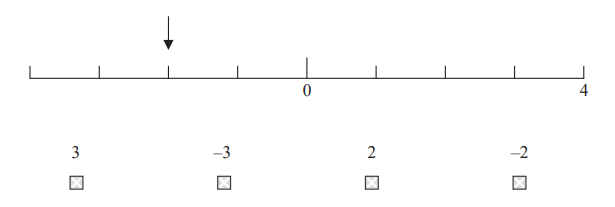
\includegraphics[width=15cm]{Numberline.png}

\begin{flushright}
    \text{ (2)}
\end{flushright}
 \vspace{10pt}

\end{document}


